\documentclass
[aps,nofootinbib,prl,showpacs,twocolumn,groupedaddress,superscriptaddress]
{revtex4}
\usepackage{graphicx} 
\usepackage{dcolumn} 
\usepackage{longtable} 
\usepackage{amssymb} 
\usepackage{bbold}
\usepackage{amsmath} 
\usepackage{amsfonts} 
\usepackage{slashed} 
\usepackage[dvipsnames]{xcolor} 
\usepackage{soul}
%=============================================================================
\def\cM{{\widehat{M}}}
\newcommand{\sube}{_\text{\tiny EX}}
\newcommand{\subd}{_\text{\tiny D}}
\def\cS{{\mathcal S}}
\newcommand*{\mprime}{^{\prime}\mkern-1.2mu}
\newcommand*{\mdprime}{^{\prime\prime}\mkern-1.2mu}
\newcommand*{\mtprime}{^{\prime\prime\prime}\mkern-1.2mu}
\newcommand{\red}[1]{\textcolor{red}{#1}}
\newcommand{\green}[1]{\textcolor{green}{#1}} 
\newcommand{\gray}[1]{\textcolor{gray}{#1}} 
\newcommand{\blue}[1]{\textcolor{blue}{#1}} 
\newcommand{\bs}[1]{\boldsymbol{#1}} 
\newcommand{\nopieft}{\mbox{$\slashed{\pi}$EFT}} 
\newcommand{\eftnopi}{\mbox{EFT($\slashed{\pi}$) }} 
\newcommand{\Lag}{{\cal L}}
\newcommand{\la}{\label} 
\newcommand{\be}{\begin{equation}} 
\newcommand{\ee}{\end{equation}} 
\newcommand{\vcl}[1]{\ensuremath{\bar{\boldsymbol{r}}_\text{\tiny #1}}}
\newcommand{\cl}[1]{\ensuremath{\bar{r}_\text{\tiny #1}}}
\newcommand{\vsp}[1]{\ensuremath{\boldsymbol{r}}_\text{\tiny #1}}
\newcommand{\rvec}{{\bs{r}}} 
\newcommand{\xvec}{{\bs{x}}} 
\newcommand{\sgmvec}{\ensuremath{\boldsymbol{\sigma}}} 
\newcommand{\tauvec}{\ensuremath{\boldsymbol{\tau}}} 
\newcommand{\half}{\frac{1}{2}}
\newcommand{\eg}{\textit{e.g.}\;}
\newcommand{\ie}{\textit{i.e.}\;}
\newcommand{\wrt}{\textit{wrt.}\;}
\newcommand{\etc}{\textit{etc.}\;}
\newcommand{\ve}[1]{\ensuremath{\boldsymbol{#1}}}
\newcommand{\ddrei}[1]{\delta_{\tiny \Lambda}^{(3)}\!\big(#1\big)}
\newcommand{\coup}[3]{\left[\,#1\,\otimes\,#2\,\right]^{#3}}
\newcommand{\threej}[6]{ \begin{pmatrix}
   #1 & #2 & #3 \\
   #4 & #5 & #6 
  \end{pmatrix}}
\newcommand{\lam}[1]{\mbox{\ensuremath{\Lambda=#1\,\text{fm}^{-1}}}}   
\usepackage{pifont}
\renewcommand\thefootnote{\ding{\numexpr171+\value{footnote}}}
\let\endtitlepage\relax
%=============================================================================

\begin{document}

\title{Derivation of an inter-cluster potential from
a two-fermion contact interaction}
\author{JK}

\date{\today}

\begin{abstract}
The potential acting between a point particle and a bound state of $A$ particles
is related to the interaction between single particles. Specifically, the
$A$-particle state is totally symmetric in coordinate space (``bosonic''), and
the single particles should be amenable to a first-order description with two-
and three-body contact/zero-range interactions. Furthermore, the internal
space of the $A+1$ equal-mass particles is given as $A$-dimensional, which
demands an $A+1$ body state of mixed symmetry. 
\end{abstract}

\maketitle


\paragraph{The inter-cluster potential}
In order to study the large-$N$ limit, we develop a model inspired by the resonating-group formalism
(\cite{Wheeler:1937zz},\cite{Wildermuth1977}).
That entails the assumption of a frozen $A$-body core whose spatially symmetric wave function we
parametrize with a single parameter $a$ via
\be\label{eq.rgm.corewfkt}
\phi_A:=e^{-\frac{a}{2}\sum_{i=1}^A\left(\ve{r}_i-\ve{R}_A\right)^2}\;\;\;;
\begin{array}{l}
     \ve{r}_i\;\;\text{\scriptsize : single-particle coordinates}  \\
     \ve{R}_A\;\;\text{\scriptsize : core centre of mass}
\end{array}\;\;.
\ee
The system is thereby reduced to only three degrees of freedom, namely the relative distance
between core and the odd particle. The respective equation of motion reads in terms of the effective
mass $\mu$, the relative kinetic energy $E$ between core and odd particle:
\be\label{eq.rgm.eqom}
\int\left\lbrace~\phi^*_A\left(-\frac{\hbar^2}{2\mu}\ve{\nabla}_R^2-E+\mathcal{V}\right)
\mathcal{A}\left[\phi_A\psi(\ve{R})\right]\right\rbrace d\ve{r}_{1\ldots A}=0\;\;.
\ee
Antisymmetrization is required between two particles only, 
$\mathcal{A}=\mathbb{1}-P_{A,A+1}$, 
and the interaction is effective, only if it involves the odd particle:
\begin{align}
\mathcal{V}=&~C_0(\Lambda)\,\sum_{i}^{A-1}\,\ddrei{\ve{r}_i-\ve{r}_{A+1}}\\
&+D_1(\Lambda)\,\sum^{A-1}_{i<j}\,\left[\ddrei{\ve{r}_i-\ve{r}_j}\,
\ddrei{\ve{r}_i-\ve{r}_{A+1}}\right.\\&\qquad\qquad\left.+
\,\ddrei{\ve{r}_i-\ve{r}_{A+1}}\,
\ddrei{\ve{r}_j-\ve{r}_{A+1}}\right]\;\,.
\end{align}
The contribution from the identical copy of the $(A+1)^\text{\scriptsize th}$ particle
-- without loss of generality identified with label $A$ -- interacting is excluded, 
because we anticipate its vanishing because of antisymmetrization.
As in our calculations, the zero-range contact forces are smeared out in order to 
obtain regular solutions -- in contrast to, \eg,
Bethe-Peierls~\cite{bethePeierls} boundary conditions 
-- this {\it a priori} exclusion introduces artefacts. We assume
that those are insignificant relative to the other terms from 
the inter-fragment interaction.

The integration in \eqref{eq.rgm.eqom} yields a three-dimensional 
Schr\"odinger equation with a non-local potential
\begin{widetext}
\be\label{eq.rgm.sglnonloc}
\left(-\frac{\hbar^2}{2\mu}\ve{\nabla}_R^2-E\right)\psi(\ve{R})+\sum_{n=1}^3\eta_n~e^{-\kappa_n\ve{R}^2}\psi(\ve{R})-
\sum_{n=1}^4\zeta_n\int\left\lbrace\mathcal{O}_ne^{-\alpha_n\ve{R}^2-\beta_n\ve{R}\cdot\ve{R}'-\gamma_n\ve{R}'^2}\right\rbrace\psi(\ve{R}') d\ve{R}'=0\;\;.
\ee
\end{widetext}
The coefficients $\alpha,\ldots,\kappa$ are functions of the number of
core particles $A$,
the core size $a$, the interaction regulator $\Lambda$,
and the single-particle mass $m$, and 
\begin{align}\la{eq.exop}
\mathcal{O}_1=&~-\frac{\hbar^2}{2\mu}\ve{\nabla}_R^2-E\\
\to&~-\frac{\hbar^2}{2\mu}\left(4\alpha_1^2\ve{R}^2+\beta_1^2\ve{R}'^2
+4\alpha_1\beta_1\ve{R}\cdot\ve{R}'-2\alpha_1\right)-E\;\;,\nonumber
\end{align}
while $\mathcal{O}_{2,3,4}=\mathbb{1}$. The sign ($+$) of the first sum -- the direct
interaction -- is that of the microscopic LEC. In contrast, the second, non-local
part reverts the sign. For example, the effect of an attractive 2-body potential
becomes a repulsive contribution due to antisymmetrization in this term.

A few comments are in order. Firstly, $\zeta_{1\ldots4}=0$ if $\mathcal{A}=\mathbb{1}$, \ie, the
inter-cluster potential is local. The first non-local term encodes the so-called exchange interaction.
It is non-zero even in the absence of inter-particle forces. The two- and three-body
contact forces affect the inter-cluster potential structurally in the same way. However, the respective
coefficients differ significantly in their dependence on $A,a$ and $\Lambda$. It is the combination
of both, the two- and three-body terms, which results in the changing character of the interaction,
the formation of attractive and repulsive regions, and thereby the possibility to bind the odd particle
to the core. We postpone a detailed analysis of the sensitivity of the inter-cluster potential,
for now, and continue with the discussion of the emerging spectrum of \eqref{eq.rgm.sglnonloc}.

\paragraph{Partial-wave projection} We solve Eq.\eqref{eq.rgm.sglnonloc} by expanding
the total wave function\footnote{Dimensionality: $[\psi]=\text{fm}^{-\frac{3}{2}}\;,\;[\phi]=\text{fm}^{-\frac{1}{2}}$}
\be
\psi(\ve{R})=R^{-1}\sum_{lm}\phi_{lm}(R)Y_{lm}(\hat{\ve{R}})\;\;
\ee
and a projection with the integral operator
\be
\int d^2\hat{\ve{R}}~Y^*_{lm}(\hat{\ve{R}})
\ee
from the left. The uncoupling of different partial waves becomes explicit when
\be
e^{-\beta\ve{R}\cdot\ve{R}'}=4\pi\sum_{LM}i^Lj_L(i\beta RR')Y^*_{LM}(\hat{\ve{R}})Y_{LM}(\hat{\ve{R}}')
\ee
is substituted. In the $n=1$ part, which encodes the exchange effect on the free
Hamiltonian, we apply the Laplacian before making the above and following
substitutions:
\be
\ve{R}\cdot\ve{R}'=-\sqrt{3}\coup{\ve{R}_p}{\ve{R}\mprime_{-p}}{00}
\ee
with $\ve{r}_m=\sqrt{\frac{4\pi}{3}}rY_{1,m}(\hat{\ve{r}})$. Using Eq.(4.6.3) and
Eq.(3.7.8) of~\cite{Edmonds}, we obtain the equation of motion for a single
partial wave:
\begin{widetext}
\begin{subequations}\la{eq.rgm.sglnonloc.pw}
\begin{gather}
\left(\frac{\hbar^2}{2\mu}\left[-\partial^2_R+\frac{l(l+1)}{R^2}\right]-E\right)
\phi_{lm}(R)\\
-(-E)\int
\left(4\pi\,i^l\cdot\zeta_1\cdot j_l(i\beta_1 RR')\right)\cdot
 e^{-\alpha_1\ve{R}^2-\gamma_1\ve{R}'^2}\phi_{lm}(R\mprime)~R\mprime dR\mprime
 \la{eq.rgm.sglnonloc.pw.Eex}\\
-\left(\frac{\hbar^2}{2\mu}\right)\int
(4\pi\cdot\zeta_1) \cdot e^{-\alpha_n\ve{R}^2-\gamma_n\ve{R}'^2}
\cdot\Bigg\lbrace
\left[-(4\alpha_1^2R^2+\beta_1^2R\mprime^2-2\alpha_1)+\frac{l(l+1)}{R^2}\right]
 i^l j_{l}(i\beta_1 RR')\nonumber\\
+(4\alpha_1\beta_1)\cdot RR\mprime\cdot
 \left(i^{l-1} j_{l-1}(i\beta_1 RR') (2l-3)
 \threej{1}{l-1}{l}{0}{0}{0}^2+
 i^{l+1} j_{l+1}(i\beta_1 RR') (2l-1)
 \threej{1}{l+1}{l}{0}{0}{0}^2\right)\Bigg\rbrace
~\phi_{lm}(R\mprime)~R\mprime dR\mprime\la{eq.rgm.sglnonloc.pw.tex}\\
-\sum_{n=\red{2}}^4\zeta_n\int
(4\pi\,i^l)\cdot j_l(i\beta_n RR')\cdot 
e^{-\alpha_n\ve{R}^2-\gamma_n\ve{R}'^2}~\phi_{lm}(R\mprime)~R\mprime\,dR\mprime\la{eq.rgm.sglnonloc.pw.noloc}\\
+\sum_{n=1}^3\eta_n~e^{-\kappa_n\ve{R}^2}\phi_{lm}(R)\la{eq.rgm.sglnonloc.pw.t}\\
 =0\;\;.\nonumber
\end{gather}
\end{subequations}
\end{widetext}
This equation defines a generalized Eigenvalue problem
\be\la{eq.rgm.gev}
\int dR\mprime~\hat{\mathcal{D}}_{RR\mprime}~\phi_{lm}(R\mprime)=
E\int dR\mprime\,\left(\delta_{RR\mprime}+\hat{\mathcal{K}}_{RR\mprime}\right)
\phi_{lm}(R\mprime)
\ee
whose solution we expand in a finite set of harmonic oscillator
functions\footnote{
$\phi_{nl\nu}(R)=N_{nl\nu}R^{l+1}e^{-\nu R^2}L_{n}^{l+1/2}(2\nu R^2)$
in terms of a normalizing constant $N_{nl\nu}=
\left(\left(\frac{2\nu^3}{\pi}\right)^{1/2}\cdot\frac{2^{2l+n+3}n!\nu^l}{(2n+2l+1)!!}\right)^{1/2}$ and generalized
Laguerre polynomials $L_n^m(x)$.
}.

\paragraph{Example: 5-body system}
In the following, we analyse features of the effective interaction for the
specific case of four internal degrees of freedom and a system of five particles
with identical masses. With the numerical values as given in table~\ref{tab.constants},
this example pertains to nuclear physics as described in leading order with the
pionless effective field theory.

\begin{table}
\be\la{tab.constants}
\setlength{\tabcolsep}{4pt}
\renewcommand{\arraystretch}{1.4}
\begin{array}{c|cccc}
n & \eta_n & \kappa_n & & \\
1 & & & & \\
2 & & & & \\
3 & & & & \\
n & \zeta_n & \alpha_n & \beta_n & \gamma_n \\
1 & & & & \\
2 & & & & \\
3 & & & & \\
4 & & & & \\
\hline
\end{array}
\ee
\caption{Numerical values which specify the core-particle motion via
Eq.~\eqref{eq.rgm.sglnonloc.pw} for $\lam{4}$, $A=4$, $m_N=938~$MeV, $a=0.56~$fm, $\hbar c=197~\text{MeV$\cdot$fm}$.}
\end{table}

\newpage


\section{Appendix: The core wave function}
Our ansatz for an $A$-boson system in its ground state
(symmetric in space \wrt particle exchange) is
\be
\phi_A:=e^{-\frac{a}{2}\sum_{i=1}^{\red{A}}\vcl{i}^2}=e^{-a\sum^{\red{A-1}}\vcl{i}^2-a\sum^{\red{A-1}}_{\red{i<j}}\vcl{i}\cdot\vcl{j}}\la{eq.wfktphi}\;\;.
\ee
Instead of single-particle coordinates, the usage of cluster coordinates identifies
the centre of mass as the origin of a ``harmonic'', effective potential, in which the
particles reside in their independent-particle/mean-field ground state. All observables
of the system in this state depend thus on a single
parameter, the (oscillator) width $a$. The root-mean-square radius, in particular, relates to
$a$ via
\begin{align}
\mathfrak{r}^2=&\frac{\int\limits_{\mathbb{R}^{3(A-1)}}d(\vcl{1},\ldots,\vcl{\red{A-1}})~
\sum_{i=1}^{\red{A-1}}\vcl{i}^2\phi_A^2}
{\int\limits_{\mathbb{R}^{3(A-1)}}d(\vcl{1},\ldots,\vcl{\red{A-1}})~\phi_A^2}\label{eq.rms}\\
=&\frac{3}{2}\cdot\frac{(A-1)^2}{A}\cdot a^{-1}\stackrel{A\gg 1}{=}
\frac{3}{2}\cdot A\cdot a^{-1}\;\;.
%=&r^2_0\cdot A^{\frac{2}{3}}
\end{align}
We assume the correlation between the radius $\mathfrak{r}$ and the ground-state wave function of the
$3$-nucleon system, to hold for any spatially symmetric $A$-boson system. However, the functional
relation, $\mathfrak{r}=f\left[A,B(3),B(2)\right]$, is unknown (to the best of our knowledge).

The numerical results obtained for $B(3)=1.5,3,4~$MeV at $B(2)=1~$MeV yield an almost
linear increase: $\mathfrak{r}\propto A$ for $A=3\ldots6$. The rate of this increase is
independent of $B(3)$, while its starting point is set by $B(3)$ -- the $\mathfrak{r}$
curve for some $B(3)$ is parallel and above all curves of smaller $B(3)$.

\begin{figure}[h] 
\centering 
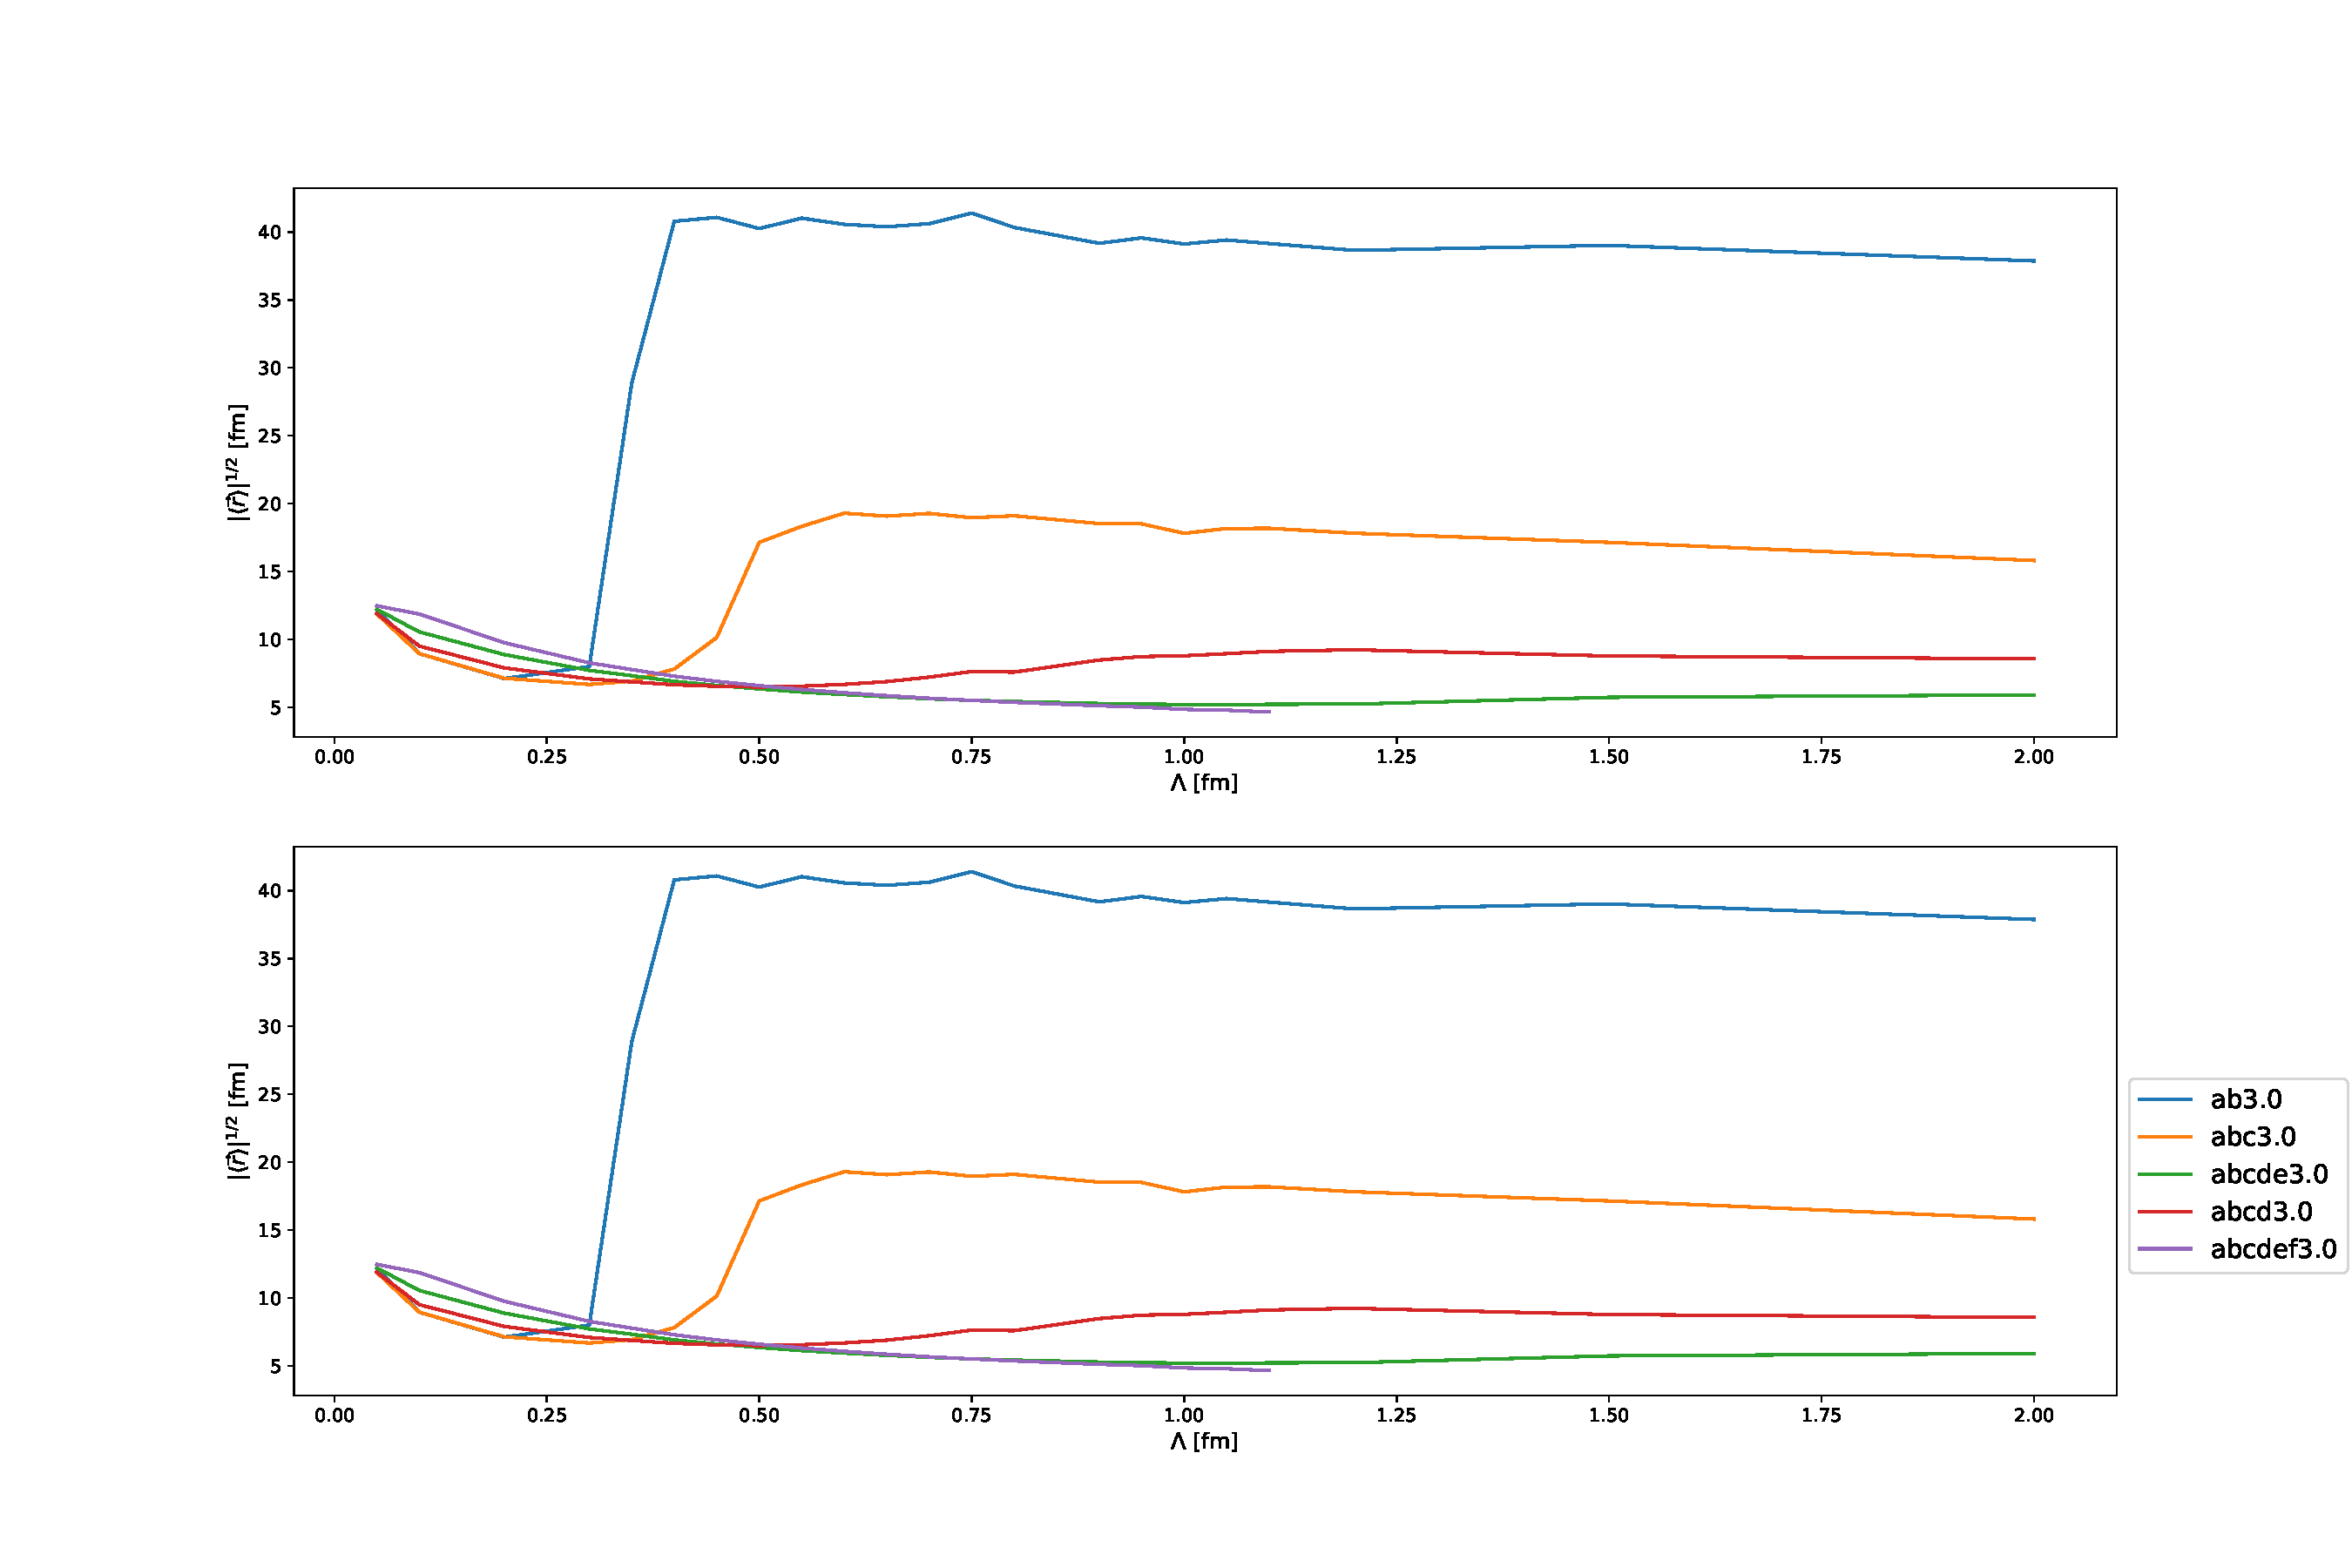
\includegraphics[width=0.5\textwidth,angle=0]{../source_python/rms_radii.pdf} 
\caption{Root-mean-square radii (defined in \eqref{eq.rms}) of a bound, $A$-boson system
for various 3-body constraints at fixed $B(2)=1~$MeV and \lam{2}.}
\label{fig.rms}
\end{figure}

Assuming instead $A$-incompressible spheres deformed into a large sphere yields
$V=\frac{4}{3}\pi \mathfrak{r}^3\propto A$ and a slower with $A$ growth of the systems.

For an appropriate parametrization of the core wave function we use the numerical values
for $A=6$ at \lam{2}: $a=\frac{25}{4}~\mathfrak{r}^{-2}=0.15$\footnote{$\mathfrak{r}(A=6,B(3)=1.5$) was calculated at \lam{1}
due to numerical hindrances at larger cutoffs. The converged value is expected to be significantly smaller, as
suggested by the outlier in Fig.\ref{fig.rms}.}$,0.65,0.90~$fm$^{-2}$.

$$
a=\left\lbrace
\begin{array}{cl} \frac{3}{2~r_{\text{drop}}}A^{2/3}  & \text{liquid drop}\\ 
                  \frac{3}{2~r_{\text{chain}}}A^{-1}  & \text{linear chain}
\end{array}\right.
$$

\newpage
\section{Appendix: Inter-cluster Potential}
Consider two compound systems, whose relative motion is much slower compared with the
motion of the particles within each of these fragments. Within an arbitrarily small
time interval, the probability of a given particle to interact/hit/overlap with another
particle is then enhanced for the partner belonging to the same compound.
\[P_{dt}(\text{intra})\gg P_{dt}(\text{inter})\]
or
\[\text{\#(internal collisions)}\gg\text{\#(inter-cluster collisions)}\;\;.\]
The relative motion of particles within each cluster is then decoupled from, {\it one}, the
relative motion \wrt~the other cluster(s), {\it and two}, the internal motion
in those. In turn, the internal structure affects cluster-relative motion.
This reasoning underlies the single-channel resonating-group approximation and
also foreshadows the non-hermitian character of the effective interaction.

\begin{gather}
\cM\subd=\begin{pmatrix}4a & & & \\ & 4a & &\multicolumn{2}{l}{\!\!\!\!(2a)_\nabla}\\
 \multicolumn{2}{c}{(2a)_\triangle} & \ddots & \\ & & & & 4a \\\end{pmatrix}
\;\;;\;\;\ve{\cS}\subd =\ve{0}\;\;;\;\;B\subd =(R-R')
\end{gather}

\newpage

\begin{widetext}
\begin{turnpage}
\begin{table}
\setlength{\tabcolsep}{4pt}
\renewcommand{\arraystretch}{2.4}
\caption{\label{tab.rgmpot}{Defining parameters of the effective potential between
a Gaussian $A$-body core, characterized via the width $a$~\eqref{eq.rgm.corewfkt},
and one {\it odd} particle (see \eqref{eq.rgm.sglnonloc}).
The 2- and 3-body LECs $C^\Lambda_0$ and $D^\Lambda_1$ are
calibrated to a 2- and 3-body symmetric bound state (see table~\ref{tab.legend}).
$A\mprime=A-1, A\mdprime=A-2, \ldots$. The coefficients $\eta_i,\zeta_i$ {\bf do}
consider non-zero interacting pair and triplet contributions from $\sum_{i<A}$ and
$\sum_{i<A\atop j<A-1}$ but {\bf not} $(-1)^{\mathfrak{p}}$.}}
\small\centering
\begin{tabular}{lc|ccc}
\hline\hline
$i$ & $\eta_i$ & $\kappa_i$ & & \\
1   & $8~C_0^\Lambda~\frac{A\mprime}{\left(4+\frac{A\mprime}{A}\frac{\Lambda^2}{a}\right)^{3/2}}$  & $\frac{A\Lambda^2}{4A+A\mprime\frac{\Lambda^2}{a}}$ \\
2   & $
\frac{32 D_1^\Lambda a^3 A\mdprime A\mprime A^{3/2}}
{\left(16 a^2 A+4 a (3 A-1) \Lambda ^2+A\mdprime \Lambda ^4\right)^{3/2}}$ &
$\frac{\Lambda ^2 \left(4 a^2 A+2 a A \Lambda ^2\right)}
{16 a^2 A+4 a (3 A-1) \Lambda ^2+A\mdprime \Lambda ^4}$ \\
3 & 
$\frac{32 D_1^\Lambda A\mdprime A\mprime}{\left(\frac{\left(4 a+\Lambda ^2\right) \left(4 a A+A\mdprime \Lambda ^2\right)}{a^2 A}\right)^{3/2}}$ & $\frac{2 a A \Lambda ^2}{4 a A+A\mdprime \Lambda ^2}$ \\
\hline
$n$ & $\zeta_i$ & $\alpha_n$ & $\beta_n$ & $\gamma_n$ \\
1 &$\frac{2 \sqrt{2}}{\left(\frac{A\mprime (A+1)^2}{a A^3}\right)^{3/2}}$&
$\frac{a \left(A^3+A\right)}{2 A\mprime (A+1)^2}$&
$\frac{2 a A^2}{A\mprime (A+1)^2}$&
$\frac{a \left(A^3+A\right)}{2 A\mprime (A+1)^2}$\\
2 & 
$ \frac{8 C_0^\Lambda a^3 A\mprime A^{9/2}}{\pi ^{3/2} (A+1)^3 \left(4 a A\mprime+A\mdprime \Lambda ^2\right)^{3/2}}  $ & 
$\frac{\text{} a A \left(4 a \left(A^2+1\right)+\left(3 A^2+A+2\right) \Lambda ^2\right)}{2 (A+1)^2 \left(4 a A\mprime+A\mdprime \Lambda ^2\right)}$&
$\frac{4 \text{} a A^2 \left(2 a+\Lambda ^2\right)}{(A+1)^2 \left(4 a A\mprime+A\mdprime \Lambda ^2\right)}$&
$\frac{a A \left(4 a \left(A^2+1\right)+\left(A^2-A+2\right) \Lambda ^2\right)}{2 (A+1)^2 \left(4 a A\mprime+A\mdprime \Lambda ^2\right)}$ \\
3 &
$\frac{32 D_1^\Lambda A\mdprime A\mprime (a A)^{9/2}}{\pi ^{3/2} (A+1)^3 \left(16 a^2 A\mprime+4 a (3 A-4) \Lambda ^2+A\mtprime \Lambda ^4\right)^{3/2}}$&
$\frac{\text{} a A \left(16 a^2 \left(A^2+1\right)+4 a \left(5 A^2+A+4\right) \Lambda ^2+\left(5 A^2+2 A+3\right) \Lambda ^4\right)}{2 (A+1)^2 \left(16 a^2 A\mprime+4 a (3 A-4) \Lambda ^2+A\mtprime \Lambda ^4\right)}$&
$\frac{2 \text{} a A^2 \left(16 a^2+16 a \Lambda ^2+3 \Lambda ^4\right)}{(A+1)^2 \left(16 a^2 A\mprime+4 a (3 A-4) \Lambda ^2+A\mtprime \Lambda ^4\right)}$&
$\frac{a A \left(16 a^2 \left(A^2+1\right)+4 a \left(3 A^2-A+4\right) \Lambda ^2+\left(A^2-2 A+3\right) \Lambda ^4\right)}{2 (A+1)^2 \left(16 a^2 A\mprime+4 a (3 A-4) \Lambda ^2+A\mtprime \Lambda ^4\right)}$\\ 
4 &
$\frac{32 D_1^\Lambda A\mdprime A\mprime}{\pi ^{3/2} \left(\frac{(A+1)^2 \left(4 a+\Lambda ^2\right) \left(4 a A\mprime+A\mtprime \Lambda ^2\right)}{a^3 A^3}\right)^{3/2}}$&
$\frac{\text{} a A \left(4 a \left(A^2+1\right)+\left(5 A^2+2 A+3\right) \Lambda ^2\right)}{2 (A+1)^2 \left(4 a A\mprime+A\mtprime \Lambda ^2\right)}$&
$\frac{2 \text{} a A^2 \left(4 a+3 \Lambda ^2\right)}{(A+1)^2 \left(4 a A\mprime+A\mtprime \Lambda ^2\right)}$&
$\frac{a A \left(4 a \left(A^2+1\right)+\left(A^2-2 A+3\right) \Lambda ^2\right)}{2 (A+1)^2 \left(4 a A\mprime+A\mtprime \Lambda ^2\right)}$\\
\end{tabular}
\end{table}
\end{turnpage}
\end{widetext}

\newpage

\bibliographystyle{unsrt}
\bibliography{Thebibliography.bib}
\end{document}
